\documentclass[10pt,border=4pt]{standalone}
\usepackage{mathptmx}
\usepackage{amsmath,amssymb,bm}
\usepackage{tikz}
\usetikzlibrary{patterns,decorations.pathmorphing,decorations.pathreplacing,arrows.meta,fit,backgrounds,calc,positioning,shapes.geometric}
\definecolor{acc}{HTML}{0B5394}
\definecolor{accl}{HTML}{EAF0F7}
\definecolor{grp}{HTML}{F5F5F5}
\definecolor{org}{HTML}{C55A11}
\definecolor{orgl}{HTML}{FBEFE6}
\tikzset{
 dat/.style={draw=black,line width=0.6pt,fill=white,align=center,font=\small,inner sep=3pt,minimum height=0.85cm},
 lay/.style={draw=acc,line width=0.8pt,fill=accl,rounded corners=2pt,align=center,font=\small,inner sep=3pt,minimum height=0.85cm},
 cnd/.style={draw=org,line width=0.8pt,fill=orgl,rounded corners=2pt,align=center,font=\small,inner sep=3pt,minimum height=0.75cm},
 op/.style={circle,draw=black,line width=0.6pt,fill=white,inner sep=0.5pt,font=\small,minimum size=5mm},
 grpb/.style={draw=black!45,dashed,line width=0.6pt,rounded corners=3pt,inner sep=6pt},
 arr/.style={-{Latex[length=2.2mm,width=1.7mm]},line width=0.7pt},
 carr/.style={-{Latex[length=2.2mm,width=1.7mm]},line width=0.7pt,draw=org},
 shp/.style={font=\scriptsize,text=black!70,inner sep=1pt},
 lab/.style={font=\footnotesize,inner sep=1pt},
 ttl/.style={font=\small\bfseries,inner sep=0pt,anchor=west}
}
\newcommand{\xh}{\mathbf{x}_h}\newcommand{\xf}{\mathbf{x}_f}

\begin{document}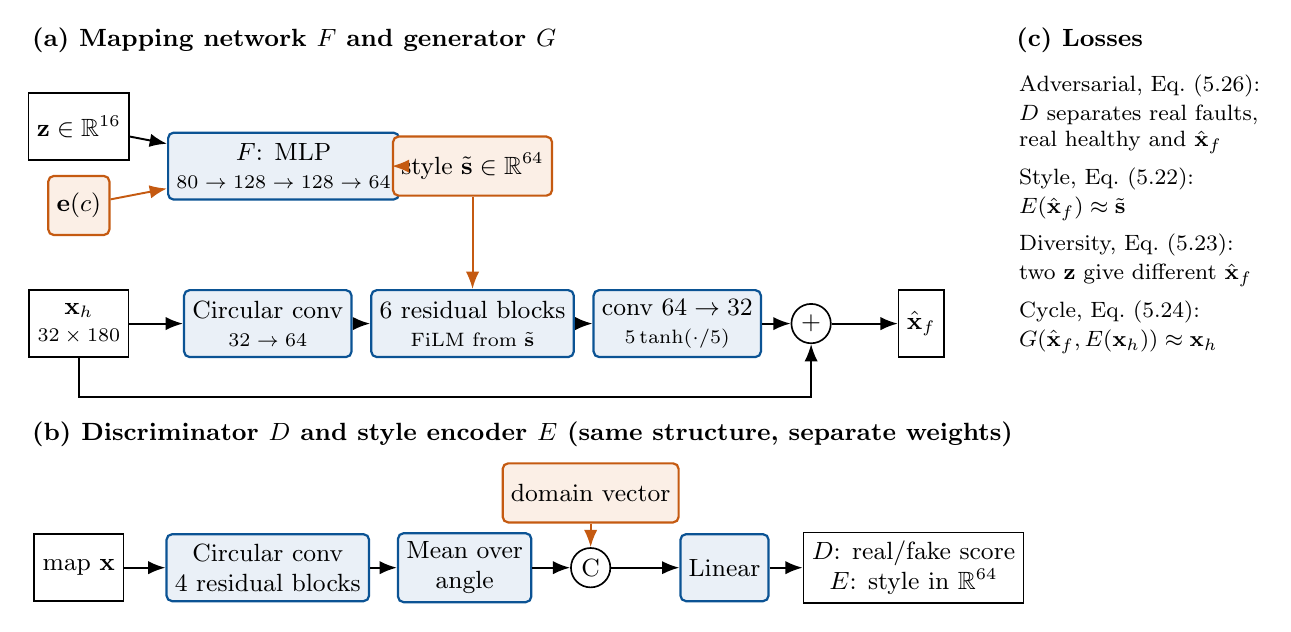
\begin{tikzpicture}[x=1cm,y=1cm]
\node[ttl] at (-0.6,1.7) {(a) Mapping network $F$ and generator $G$};
\node[dat] (z) at (0,0.6) {$\mathbf{z}\in\mathbb{R}^{16}$};
\node[cnd] (e) at (0,-0.4) {$\mathbf{e}(c)$};
\node[lay] (F) at (2.6,0.1) {$F$: MLP\\[-1pt]\scriptsize $80\to128\to128\to64$};
\node[cnd] (s) at (5.0,0.1) {style $\tilde{\mathbf{s}}\in\mathbb{R}^{64}$};
\draw[arr] (z)--(F); \draw[carr] (e)--(F); \draw[carr] (F)--(s);
\node[dat] (xh) at (0,-1.9) {$\xh$\\[-1pt]\scriptsize $32\times180$};
\node[lay] (g1) at (2.4,-1.9) {Circular conv\\[-1pt]\scriptsize $32\to64$};
\node[lay] (g2) at (5.0,-1.9) {6 residual blocks\\[-1pt]\scriptsize FiLM from $\tilde{\mathbf{s}}$};
\node[lay] (g3) at (7.6,-1.9) {conv $64\to32$\\[-1pt]\scriptsize $5\tanh(\cdot/5)$};
\node[op] (ad) at (9.3,-1.9) {$+$};
\node[dat] (xg) at (10.7,-1.9) {$\hat{\mathbf{x}}_f$};
\draw[arr] (xh)--(g1); \draw[arr] (g1)--(g2); \draw[arr] (g2)--(g3); \draw[arr] (g3)--(ad); \draw[arr] (ad)--(xg); \draw[carr] (s)--(g2);
\draw[arr] (xh.south) -- ++(0,-0.5) -| (ad.south);
% (b) D and E
\node[ttl] at (-0.6,-3.3) {(b) Discriminator $D$ and style encoder $E$ (same structure, separate weights)};
\node[dat] (x) at (0,-5.0) {map $\mathbf{x}$};
\node[lay] (d1) at (2.4,-5.0) {Circular conv\\4 residual blocks};
\node[lay] (d2) at (4.9,-5.0) {Mean over\\angle};
\node[op] (cat) at (6.5,-5.0) {C};
\node[cnd] (dom) at (6.5,-4.05) {domain vector};
\node[lay] (d3) at (8.2,-5.0) {Linear};
\node[dat] (o) at (10.6,-5.0) {$D$: real/fake score\\$E$: style in $\mathbb{R}^{64}$};
\draw[arr] (x)--(d1); \draw[arr] (d1)--(d2); \draw[arr] (d2)--(cat); \draw[carr] (dom)--(cat); \draw[arr] (cat)--(d3); \draw[arr] (d3)--(o);
% (c) losses
\node[ttl] at (11.9,1.7) {(c) Losses};
\node[lab,align=left,anchor=north west] at (11.9,1.3) {Adversarial, Eq.~(5.26):\\[1pt]$D$ separates real faults,\\real healthy and $\hat{\mathbf{x}}_f$\\[4pt]Style, Eq.~(5.22):\\[1pt]$E(\hat{\mathbf{x}}_f)\approx\tilde{\mathbf{s}}$\\[4pt]Diversity, Eq.~(5.23):\\[1pt]two $\mathbf{z}$ give different $\hat{\mathbf{x}}_f$\\[4pt]Cycle, Eq.~(5.24):\\[1pt]$G(\hat{\mathbf{x}}_f,E(\xh))\approx\xh$};
\end{tikzpicture}\end{document}
